
%%%%%%%%%%%%%%%%
% Segmentation %
%%%%%%%%%%%%%%%%

\section{Segmentation}
\label{sec:segm}


\subsection{Binary segmentation network}

This section discusses a deep convolutional binary segmentation network, based largely on the autoencoder described in section \textcolor{blue}{\ref{sec:auto2}}. To train the model, a subset of the full dataset was used (see \textcolor{blue}{\ref{sec:intro}} for details). In accordance with the assignment, training labels were binarized. This was accomplished by converting the segmented images to grayscale and applying a threshold of .02 to the pixel values. This made sure that only the black pixels remained $0$, and all the others were set to $1$. Throughout this section, I'll refer to the 1-values as 'foreground', and the 0-values as 'background'.

\begin{figure}[!htbp]
  \begin{center}
    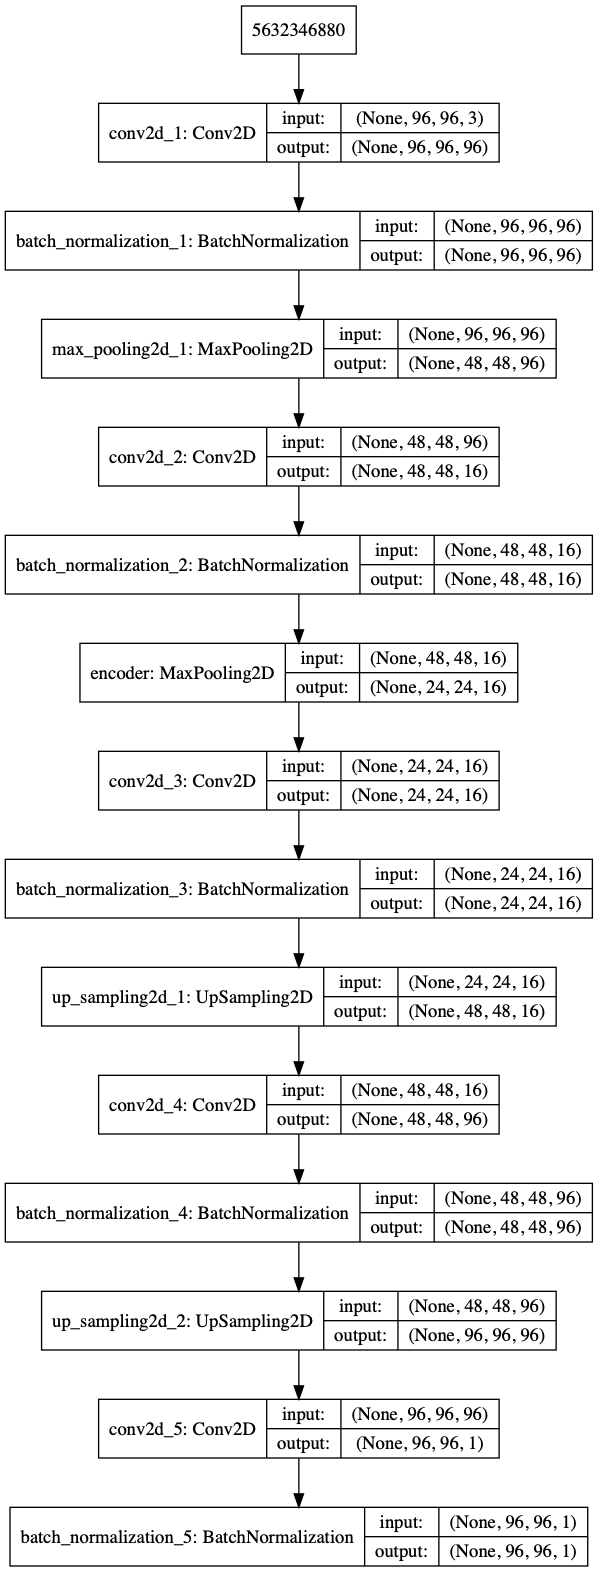
\includegraphics[height=20cm, keepaspectratio]{images/segm_architecture}
    \caption{Deep convolutional architecture for the segmentation network. Input dimensions are $96 \times 96 \times 3$. The model predicts a score per pixel position, ignoring color channels---hence the output dimensions are $96 \times 96 \times 1$.}
    \label{fig:segm_architecture}
  \end{center}
\end{figure}

\paragraph{Architecture} The architecture of the segmentation network is shown in \ref{fig:segm_architecture}. It is very closely related to the DCA architecture (see figure \textcolor{blue}{\ref{fig:auto2}}, except for a few minor changes. More explicitly, the number of filters in the convolutional layers was increased in an effort to capture more information. This decision was made after some experimentation---the impact is likely to be on the smaller end. The model gives fair results, however, hence this architecture was kept. The kernel values were initialized in a random uniform manner, and bias was initialized to zero. Again, all activation functions were \textit{ReLU}, save the final activation, where a \textit{sigmoid} was used to obtain values in the $[0,1]$ range.

\paragraph{Network parameters} As was the case in sections \textcolor{blue}{\ref{sec:auto}} and \textcolor{blue}{\ref{sec:class}}, training was done using the \textit{Adam} optimizer algorithm. The loss function was \textit{mean squared error}, as was the case with the autoencoder models. Due to the larger amount of trainable parameters, the number of training epochs was set to 500---a fairly high number. The early stopping criterion was set to 50 epochs without validation loss improvement. This criterion was purposely set to a very lenient value, after observing several training attempts and noticing a significant variability in the validation loss progression.

\begin{figure}[!htbp]
  \begin{center}
    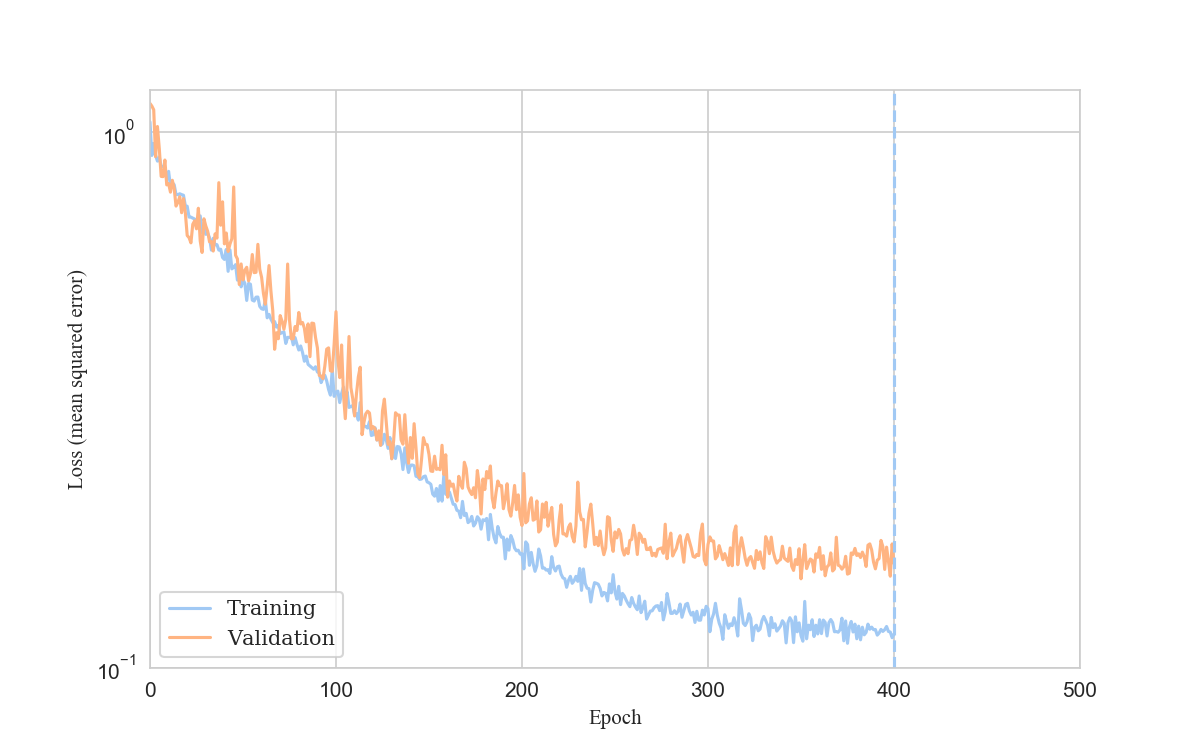
\includegraphics[width=\linewidth, keepaspectratio]{images/segm_history}
    \caption{Training history for the segmentation network. The y-axis represents the loss value (mean squared error). The vertical dotted line indicates when early stopping occurred, due to a lack of improvement in the latter value. Loss is expressed on a logarithmic scale.}
    \label{fig:segm_history}
  \end{center}
\end{figure}

\paragraph{Evaluation} The training process is visualized in figure \textcolor{blue}{\ref{fig:segm_history}}. The graph suggests that some improvement was still possible, but overtraining would become a real risk. Figure \textcolor{blue}{\ref{fig:segm_prediction}} shows how the network segmented a random selection of (previously unseen) test images. The average loss for each of the datasets is shown in table \textcolor{blue}{\ref{tab:segm_eval}}. It shows how the model is better accustomed to the training data, but not overly biased towards the validation images.

\begin{figure}[!htbp]
  \begin{center}
    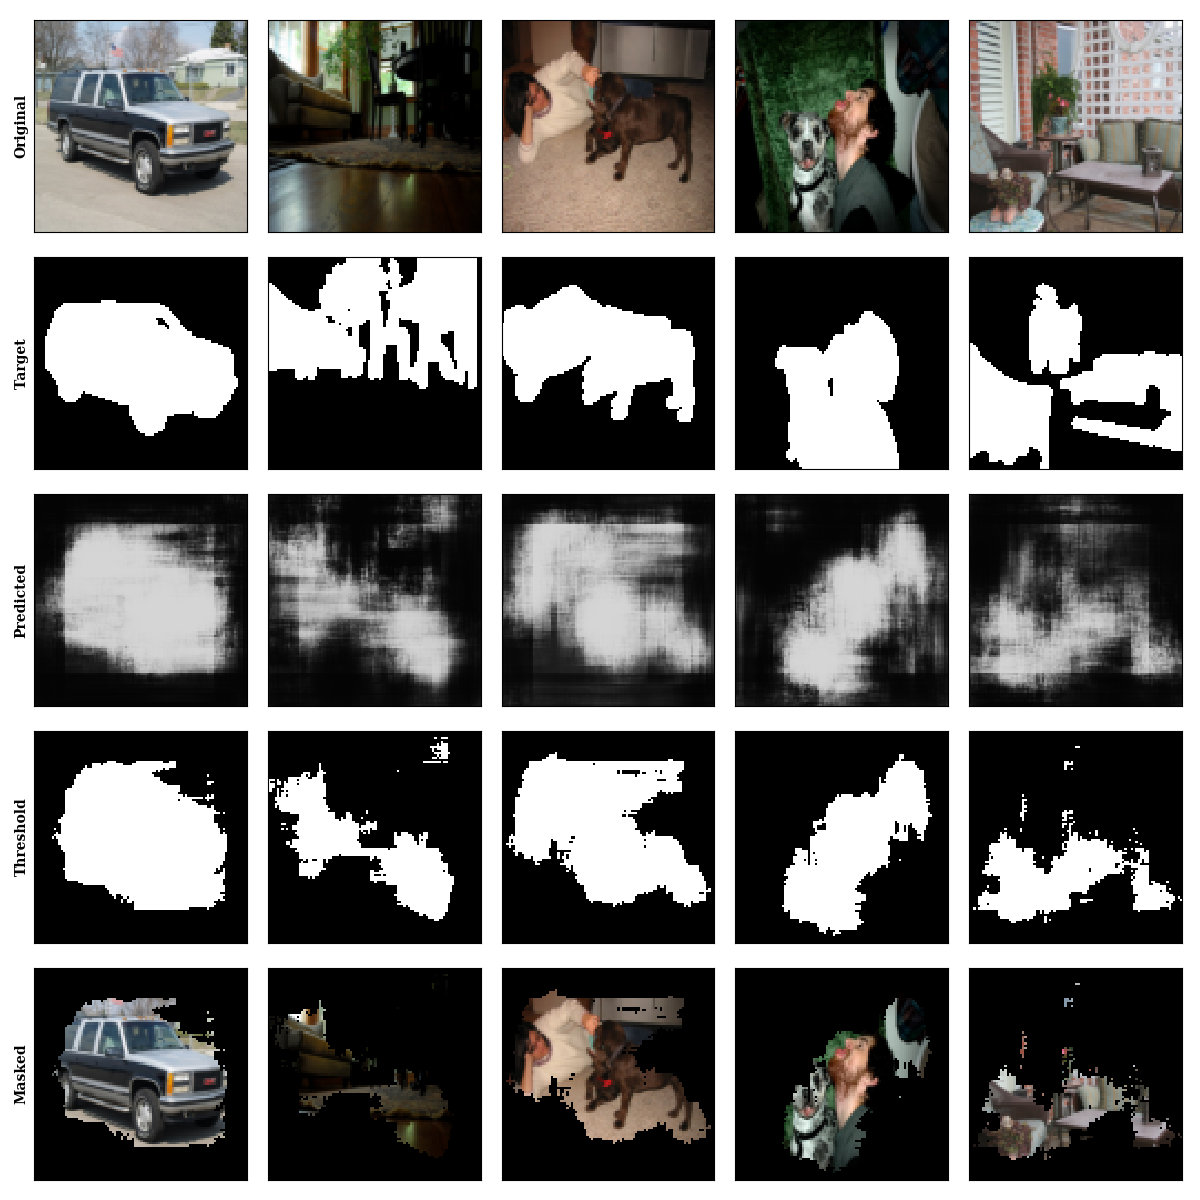
\includegraphics[width=\linewidth, keepaspectratio]{images/segm_prediction}
    \caption{Segmentation given by network for a random selection of 5 'fresh' test images ($96\times96\times3$ pixels). The top row shows the original images. The second row shows the binarized segmentation labels. The middle row shows the model output for the source images. The second to last row shows binarized predictions (threshold = $0.5$). The bottom row, finally, uses the binarized prediction as a mask over the source image.}
    \label{fig:segm_prediction}
  \end{center}
\end{figure}



\begin{table}[!htbp]

  \renewcommand{\arraystretch}{1.5}
  \centering

  \begin{tabular}{@{}cccc@{}}

    \toprule
    Model                                  & \textbf{Train} & \textbf{Validation} & \textbf{Test} \\ \midrule
    \textbf{\textit{Segmentation network}} & \num{9.32e-2}  & \num{1.50e-1}       & \num{1.43e-1} \\\bottomrule
  \end{tabular}
  \caption{Evaluation of segmentation model based on reconstruction loss: \textit{mean squared error} values for training, validation and test datasets.}
  \label{tab:segm_eval}
\end{table}

\subsection{Reflection}


% Make it better by combining results with edge detection and morphological operations to fill gaps, or just overlaying rectangles on outer edges.

% Interesting: picture of training 